\lstinputlisting[language=bash,basicstyle=\small]{python_codes/fieldstone_102/keywords}

\begin{center}
Code at \url{https://github.com/cedrict/fieldstone/tree/master/python_codes/fieldstone_102}
\end{center}

\par\noindent\rule{\textwidth}{0.4pt}

%%%%%%%%%%%%%%%%%%%%%%%%%%%%%%%%%%%%%%%%%%%%%%%%%%%%%%%%%%%%%%%%%%%%%%%%%%%%%%%%%%%%%%%%%%%%%%%%%%%%

\begin{center}

\includegraphics[width=1cm]{images/fortran/fortran} 
\end{center}

This stone is a 'simple' approach to the implementation of Conformal Refinement. The code was written 
a few years prior to my working on fieldstone, so it is in Fortran. 

Let us start with a very simple test: the mesh counts $9\times 7=63$ elements.
The greyed elements are those to be refined. We then first flag the nodes which compose them and these are shown in teal color.
Based on this information we can then consider each element in the mesh and assign it a type, based on whether or not one or more nodes are flagged:

\begin{center}
\begin{flushright} {\tiny {\color{gray} (tikz\_cr\_1.tex)}} \end{flushright}
%~~~~~~~~~~~~~~~~~~~~~~~~~~~~~~~~~~~~~~~~~~~~~~~~~~~~~~~~~~~~~~~~~~~~~~~~~~~~~~~~~~~~~~~~~~~~~~~~~~


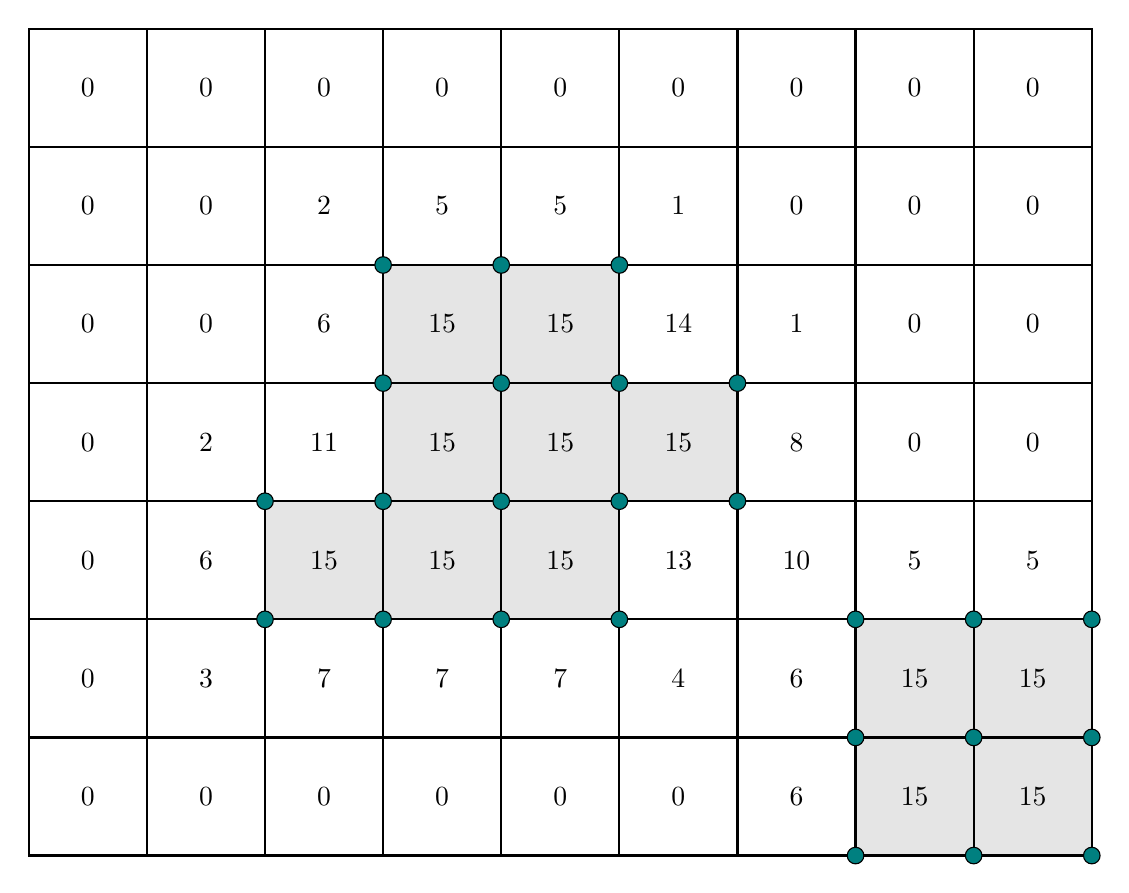
\begin{tikzpicture}
%\draw[step=0.5cm,gray,very thin] (0,0) grid (14,11); 

\draw[fill=gray!20](3,3) rectangle (7.5,4.5);  
\draw[fill=gray!20](4.5,4.5) rectangle (7.5,7.5);  
\draw[fill=gray!20](7.5,4.5) rectangle (9,6);  
\draw[fill=gray!20](10.5,0) rectangle (13.5,3);  

\draw[thick](0,0) rectangle (13.5,10.5);
\draw[thick](0,1.5)--(13.5,1.5);
\draw[thick](0,3)--(13.5,3);
\draw[thick](0,4.5)--(13.5,4.5);
\draw[thick](0,6)--(13.5,6);
\draw[thick](0,7.5)--(13.5,7.5);
\draw[thick](0,9)--(13.5,9);

\draw[thick](1.5,0)--(1.5,10.5);
\draw[thick](3,0)--(3,10.5);
\draw[thick](4.5,0)--(4.5,10.5);
\draw[thick](6,0)--(6,10.5);
\draw[thick](7.5,0)--(7.5,10.5);
\draw[thick](9,0)--(9,10.5);
\draw[thick](10.5,0)--(10.5,10.5);
\draw[thick](12,0)--(12,10.5);

\node[] at (0.75,0.75) {$0$};
\node[] at (2.25,0.75) {$0$};
\node[] at (3.75,0.75) {$0$};
\node[] at (5.25,0.75) {$0$};
\node[] at (6.75,0.75) {$0$};
\node[] at (8.25,0.75) {$0$};
\node[] at (9.75,0.75) {$6$};
\node[] at (11.25,0.75) {$15$};
\node[] at (12.75,0.75) {$15$};

\node[] at (0.75,2.25) {$0$};
\node[] at (2.25,2.25) {$3$};
\node[] at (3.75,2.25) {$7$};
\node[] at (5.25,2.25) {$7$};
\node[] at (6.75,2.25) {$7$};
\node[] at (8.25,2.25) {$4$};
\node[] at (9.75,2.25) {$6$};
\node[] at (11.25,2.25) {$15$};
\node[] at (12.75,2.25) {$15$};

\node[] at (0.75,3.75) {$0$};
\node[] at (2.25,3.75) {$6$};
\node[] at (3.75,3.75) {$15$};
\node[] at (5.25,3.75) {$15$};
\node[] at (6.75,3.75) {$15$};
\node[] at (8.25,3.75) {$13$};
\node[] at (9.75,3.75) {$10$};
\node[] at (11.25,3.75) {$5$};
\node[] at (12.75,3.75) {$5$};

\node[] at (0.75,5.25) {$0$};
\node[] at (2.25,5.25) {$2$};
\node[] at (3.75,5.25) {$11$};
\node[] at (5.25,5.25) {$15$};
\node[] at (6.75,5.25) {$15$};
\node[] at (8.25,5.25) {$15$};
\node[] at (9.75,5.25) {$8$};
\node[] at (11.25,5.25) {$0$};
\node[] at (12.75,5.25) {$0$};

\node[] at (0.75,6.75) {$0$};
\node[] at (2.25,6.75) {$0$};
\node[] at (3.75,6.75) {$6$};
\node[] at (5.25,6.75) {$15$};
\node[] at (6.75,6.75) {$15$};
\node[] at (8.25,6.75) {$14$};
\node[] at (9.75,6.75) {$1$};
\node[] at (11.25,6.75) {$0$};
\node[] at (12.75,6.75) {$0$};

\node[] at (0.75,8.25) {$0$};
\node[] at (2.25,8.25) {$0$};
\node[] at (3.75,8.25) {$2$};
\node[] at (5.25,8.25) {$5$};
\node[] at (6.75,8.25) {$5$};
\node[] at (8.25,8.25) {$1$};
\node[] at (9.75,8.25) {$0$};
\node[] at (11.25,8.25) {$0$};
\node[] at (12.75,8.25) {$0$};

\node[] at (0.75,9.75) {$0$};
\node[] at (2.25,9.75) {$0$};
\node[] at (3.75,9.75) {$0$};
\node[] at (5.25,9.75) {$0$};
\node[] at (6.75,9.75) {$0$};
\node[] at (8.25,9.75) {$0$};
\node[] at (9.75,9.75) {$0$};
\node[] at (11.25,9.75) {$0$};
\node[] at (12.75,9.75) {$0$};







\draw[black,fill=teal] (3,3) circle (3pt);
\draw[black,fill=teal] (4.5,3) circle (3pt);
\draw[black,fill=teal] (6,3) circle (3pt);
\draw[black,fill=teal] (7.5,3) circle (3pt);
\draw[black,fill=teal] (10.5,3) circle (3pt);
\draw[black,fill=teal] (12,3) circle (3pt);
\draw[black,fill=teal] (13.5,3) circle (3pt);
\draw[black,fill=teal] (10.5,1.5) circle (3pt);
\draw[black,fill=teal] (12,1.5) circle (3pt);
\draw[black,fill=teal] (13.5,1.5) circle (3pt);
\draw[black,fill=teal] (10.5,0) circle (3pt);
\draw[black,fill=teal] (12,0) circle (3pt);
\draw[black,fill=teal] (13.5,0) circle (3pt);
\draw[black,fill=teal] (3,4.5) circle (3pt);
\draw[black,fill=teal] (4.5,4.5) circle (3pt);
\draw[black,fill=teal] (6,4.5) circle (3pt);
\draw[black,fill=teal] (7.5,4.5) circle (3pt);
\draw[black,fill=teal] (9,4.5) circle (3pt);
\draw[black,fill=teal] (4.5,6) circle (3pt);
\draw[black,fill=teal] (6,6) circle (3pt);
\draw[black,fill=teal] (7.5,6) circle (3pt);
\draw[black,fill=teal] (9,6) circle (3pt);
\draw[black,fill=teal] (4.5,7.5) circle (3pt);
\draw[black,fill=teal] (6,7.5) circle (3pt);
\draw[black,fill=teal] (7.5,7.5) circle (3pt);


\end{tikzpicture}

\end{center}

The type is stored in the elemental array {\tt crtype} while the nodes belonging to elements to be refined are stored in {\tt crnode}.
The types are as follows:

\begin{center}
\begin{flushright} {\tiny {\color{gray} (tikz\_cr\_2.tex)}} \end{flushright}
%~~~~~~~~~~~~~~~~~~~~~~~~~~~~~~~~~~~~~~~~~~~~~~~~~~~~~~~~~~~~~~~~~~~~~~~~~~~~~~~~~~~~~~~~~~~~~~~~~~

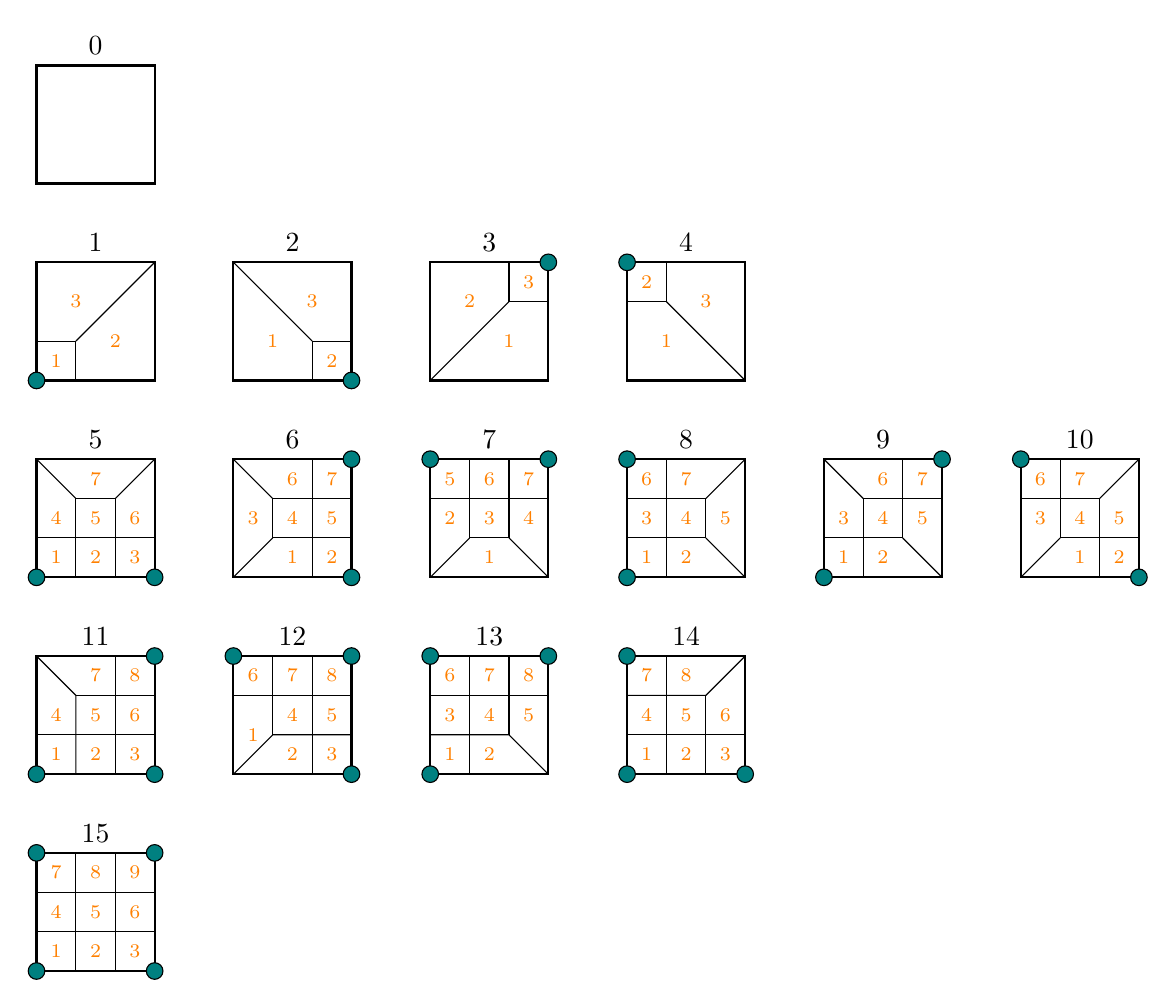
\begin{tikzpicture}
%\draw[step=1cm,gray,very thin] (0,0) grid (17,13); 

%.............................
\node[] at (1.25,12.25) {$0$};
\draw[thick](0.5,10.5) rectangle (2,12); %0

%.............................
\node[] at (1.25,9.75) {$1$};
\draw[thick](0.5,8) rectangle (2,9.5);   %1
\draw[black,fill=teal] (0.5,8) circle (3pt);
\draw[](1,8.5)--(2,9.5);   
\draw[](0.5,8.5)--(1,8.5)--(1,8);   

\node[] at (0.75,8.25) {\scriptsize \color{orange} 1};
\node[] at (1.5,8.5) {\scriptsize \color{orange} 2};
\node[] at (1,9) {\scriptsize \color{orange} 3};

%.............................
\node[] at (3.75,9.75) {$2$};
\draw[thick](3,8) rectangle (4.5,9.5); %2
\draw[black,fill=teal] (4.5,8) circle (3pt);
\draw[](4,8)--(4,8.5)--(4.5,8.5);
\draw[](3,9.5)--(4,8.5);
\node[] at (3.5,8.5) {\scriptsize \color{orange} 1};
\node[] at (4.25,8.25) {\scriptsize \color{orange} 2};
\node[] at (4,9) {\scriptsize \color{orange} 3};


%.............................
\node[] at (6.25,9.75) {$3$};
\draw[thick](5.5,8) rectangle (7,9.5); %3
\draw[black,fill=teal] (7,9.5) circle (3pt);
\draw[](5.5,8)--(6.5,9);
\draw[](6.5,9.5)--(6.5,9)--(7,9);
\node[] at (6.5,8.5) {\scriptsize \color{orange} 1};
\node[] at (6,9) {\scriptsize \color{orange} 2};
\node[] at (6.75,9.25) {\scriptsize \color{orange} 3};


%.............................
\node[] at (8.75,9.75) {$4$};
\draw[thick](8,8) rectangle (9.5,9.5); %4
\draw[black,fill=teal] (8,9.5) circle (3pt);
\draw[](8,9)--(8.5,9)--(8.5,9.5);
\draw[](8.5,9)--(9.5,8);
\node[] at (8.5,8.5) {\scriptsize \color{orange} 1};
\node[] at (8.25,9.25) {\scriptsize \color{orange} 2};
\node[] at (9,9) {\scriptsize \color{orange} 3};


%.............................
\node[] at (1.25,7.25) {$5$};
\draw[thick](0.5,5.5) rectangle (2,7);   %5
\draw[](0.5,6)--(2,6);
\draw[](1,5.5)--(1,6.5)--(1.5,6.5)--(1.5,5.5);
\draw[](0.5,7)--(1,6.5);
\draw[](2,7)--(1.5,6.5);
\draw[black,fill=teal] (0.5,5.5) circle (3pt);
\draw[black,fill=teal] (2,5.5) circle (3pt);

\node[] at (0.75,5.75) {\scriptsize \color{orange} 1};
\node[] at (1.25,5.75) {\scriptsize \color{orange} 2};
\node[] at (1.75,5.75) {\scriptsize \color{orange} 3};
\node[] at (0.75,6.25) {\scriptsize \color{orange} 4};
\node[] at (1.25,6.25) {\scriptsize \color{orange} 5};
\node[] at (1.75,6.25) {\scriptsize \color{orange} 6};
\node[] at (1.25,6.75) {\scriptsize \color{orange} 7};

%.............................
\node[] at (3.75,7.25) {$6$};
\draw[thick](3,5.5) rectangle (4.5,7);   %6
\draw[](4,5.5)--(4,7);
\draw[](4.5,6.5)--(3.5,6.5)--(3.5,6)--(4.5,6);
\draw[](3,5.5)--(3.5,6);
\draw[](3,7)--(3.5,6.5);
\draw[black,fill=teal] (4.5,5.5) circle (3pt);
\draw[black,fill=teal] (4.5,7) circle (3pt);

\node[] at (3.75,5.75) {\scriptsize \color{orange} 1};
\node[] at (4.25,5.75) {\scriptsize \color{orange} 2};
\node[] at (3.25,6.25) {\scriptsize \color{orange} 3};
\node[] at (3.75,6.25) {\scriptsize \color{orange} 4};
\node[] at (4.25,6.25) {\scriptsize \color{orange} 5};
\node[] at (3.75,6.75) {\scriptsize \color{orange} 6};
\node[] at (4.25,6.75) {\scriptsize \color{orange} 7};


%.............................
\node[] at (6.25,7.25) {$7$};
\draw[thick](5.5,5.5) rectangle (7,7);   %7
\draw[](5.5,6.5)--(7,6.5);
\draw[](6,7)--(6,6)--(6.5,6)--(6.5,7);
\draw[](5.5,5.5)--(6,6);
\draw[](7,5.5)--(6.5,6);
\draw[black,fill=teal] (5.5,7) circle (3pt);
\draw[black,fill=teal] (7,7) circle (3pt);


\node[] at (6.25,5.75) {\scriptsize \color{orange} 1};
\node[] at (5.75,6.25) {\scriptsize \color{orange} 2};
\node[] at (6.25,6.25) {\scriptsize \color{orange} 3};
\node[] at (6.75,6.25) {\scriptsize \color{orange} 4};
\node[] at (5.75,6.75) {\scriptsize \color{orange} 5};
\node[] at (6.25,6.75) {\scriptsize \color{orange} 6};
\node[] at (6.75,6.75) {\scriptsize \color{orange} 7};



%.............................
\node[] at (8.75,7.25) {$8$};
\draw[thick](8,5.5) rectangle (9.5,7);   %8
\draw[](8.5,5.5)--(8.5,7);
\draw[](8,6)--(9,6)--(9,6.5)--(8,6.5);
\draw[](9,6.5)--(9.5,7);
\draw[](9,6)--(9.5,5.5);
\draw[black,fill=teal] (8,5.5) circle (3pt);
\draw[black,fill=teal] (8,7) circle (3pt);

\node[] at (8.25,5.75) {\scriptsize \color{orange} 1};
\node[] at (8.75,5.75) {\scriptsize \color{orange} 2};
\node[] at (8.25,6.25) {\scriptsize \color{orange} 3};
\node[] at (8.75,6.25) {\scriptsize \color{orange} 4};
\node[] at (9.25,6.25) {\scriptsize \color{orange} 5};
\node[] at (8.25,6.75) {\scriptsize \color{orange} 6};
\node[] at (8.75,6.75) {\scriptsize \color{orange} 7};


%.............................
\node[] at (11.25,7.25) {$9$};
\draw[thick](10.5,5.5) rectangle (12,7);   %9

\draw[](10.5,7)--(11,6.5);
\draw[](11.5,6)--(12,5.5);
\draw[](11,6.5)--(11.5,6.5)--(11.5,6)--(11,6)--cycle;
\draw[](11.5,7)--(11.5,6.5)--(12,6.5);
\draw[](10.5,6)--(11,6)--(11,5.5);

\draw[black,fill=teal] (10.5,5.5) circle (3pt);
\draw[black,fill=teal] (12,7) circle (3pt);

\node[] at (10.75,5.75) {\scriptsize \color{orange} 1};
\node[] at (11.25,5.75) {\scriptsize \color{orange} 2};
\node[] at (10.75,6.25) {\scriptsize \color{orange} 3};
\node[] at (11.25,6.25) {\scriptsize \color{orange} 4};
\node[] at (11.75,6.25) {\scriptsize \color{orange} 5};
\node[] at (11.25,6.75) {\scriptsize \color{orange} 6};
\node[] at (11.75,6.75) {\scriptsize \color{orange} 7};



%.............................
\node[] at (13.75,7.25) {$10$};
\draw[thick](13,5.5) rectangle (14.5,7);   %10

\draw[](14,5.5)--(14,6)--(14.5,6);
\draw[](13,6.5)--(13.5,6.5)--(13.5,7);
\draw[](13.5,6.5)--(14,6.5)--(14,6)--(13.5,6)--cycle;
\draw[](13,5.5)--(13.5,6);
\draw[](14,6.5)--(14.5,7);

\draw[black,fill=teal] (14.5,5.5) circle (3pt);
\draw[black,fill=teal] (13,7) circle (3pt);

\node[] at (13.75,5.75) {\scriptsize \color{orange} 1};
\node[] at (14.25,5.75) {\scriptsize \color{orange} 2};
\node[] at (13.25,6.25) {\scriptsize \color{orange} 3};
\node[] at (13.75,6.25) {\scriptsize \color{orange} 4};
\node[] at (14.25,6.25) {\scriptsize \color{orange} 5};
\node[] at (13.25,6.75) {\scriptsize \color{orange} 6};
\node[] at (13.75,6.75) {\scriptsize \color{orange} 7};


%.............................
\node[] at (1.25,4.75) {$11$};
\draw[thick](0.5,3) rectangle (2,4.5);   %11
\draw[black,fill=teal] (0.5,3) circle (3pt);
\draw[black,fill=teal] (2,3) circle (3pt);
\draw[black,fill=teal] (2,4.5) circle (3pt);
\draw[](0.5,3.5)-- (2,3.5);
\draw[](1,4)-- (2,4);
\draw[](0.5,4.5)-- (1,4)--(1,3);
\draw[](1.5,3)-- (1.5,4.5);

\node[] at (0.75,3.25) {\scriptsize \color{orange} 1};
\node[] at (1.25,3.25) {\scriptsize \color{orange} 2};
\node[] at (1.75,3.25) {\scriptsize \color{orange} 3};
\node[] at (0.75,3.75) {\scriptsize \color{orange} 4};
\node[] at (1.25,3.75) {\scriptsize \color{orange} 5};
\node[] at (1.75,3.75) {\scriptsize \color{orange} 6};
\node[] at (1.25,4.25) {\scriptsize \color{orange} 7};
\node[] at (1.75,4.25) {\scriptsize \color{orange} 8};



%.............................
\node[] at (3.75,4.75) {$12$};
\draw[thick](3,3) rectangle (4.5,4.5);   %12
\draw[](3,3)-- (3.5,3.5)--(4.5,3.5);
\draw[](4,4.5)--(4,3);
\draw[](3,4)--(4.5,4);
\draw[](3.5,4.5)--(3.5,3.5);
\draw[black,fill=teal] (3,4.5) circle (3pt);
\draw[black,fill=teal] (4.5,3) circle (3pt);
\draw[black,fill=teal] (4.5,4.5) circle (3pt);

\node[] at (3.25,3.5)  {\scriptsize \color{orange} 1};
\node[] at (3.75,3.25) {\scriptsize \color{orange} 2};
\node[] at (4.25,3.25) {\scriptsize \color{orange} 3};
\node[] at (3.75,3.75) {\scriptsize \color{orange} 4};
\node[] at (4.25,3.75) {\scriptsize \color{orange} 5};
\node[] at (3.25,4.25) {\scriptsize \color{orange} 6};
\node[] at (3.75,4.25) {\scriptsize \color{orange} 7};
\node[] at (4.25,4.25) {\scriptsize \color{orange} 8};


%.............................
\node[] at (6.25,4.75) {$13$};
\draw[thick](5.5,3) rectangle (7,4.5);   %13

\draw[](5.5,4)--(7,4);
\draw[](5.5,3.5)--(6.5,3.5)--(7,3);
\draw[](6.5,4.5)--(6.5,3.5);
\draw[](6,4.5)--(6,3);

\draw[black,fill=teal] (5.5,3) circle (3pt);
\draw[black,fill=teal] (5.5,4.5) circle (3pt);
\draw[black,fill=teal] (7,4.5) circle (3pt);

\node[] at (5.75,3.25) {\scriptsize \color{orange} 1};
\node[] at (6.25,3.25) {\scriptsize \color{orange} 2};
\node[] at (5.75,3.75) {\scriptsize \color{orange} 3};
\node[] at (6.25,3.75) {\scriptsize \color{orange} 4};
\node[] at (6.75,3.75) {\scriptsize \color{orange} 5};
\node[] at (5.75,4.25) {\scriptsize \color{orange} 6};
\node[] at (6.25,4.25) {\scriptsize \color{orange} 7};
\node[] at (6.75,4.25) {\scriptsize \color{orange} 8};



%.............................
\node[] at (8.75,4.75) {$14$};
\draw[thick](8,3) rectangle (9.5,4.5);   %14
\draw[black,fill=teal] (8,4.5) circle (3pt);
\draw[black,fill=teal] (8,3) circle (3pt);
\draw[black,fill=teal] (9.5,3) circle (3pt);
\draw[](8,3.5) -- (9.5,3.5);
\draw[](8,4) -- (9,4)--(9.5,4.5);
\draw[](9,3) -- (9,4);
\draw[](8.5,3) -- (8.5,4.5);

\node[] at (8.25,3.25) {\scriptsize \color{orange} 1};
\node[] at (8.75,3.25) {\scriptsize \color{orange} 2};
\node[] at (9.25,3.25) {\scriptsize \color{orange} 3};
\node[] at (8.25,3.75) {\scriptsize \color{orange} 4};
\node[] at (8.75,3.75) {\scriptsize \color{orange} 5};
\node[] at (9.25,3.75) {\scriptsize \color{orange} 6};
\node[] at (8.25,4.25) {\scriptsize \color{orange} 7};
\node[] at (8.75,4.25) {\scriptsize \color{orange} 8};

%.............................
\node[] at (1.25,2.25) {$15$};
\draw[thick](0.5,0.5) rectangle (2,2);   %15
\draw[black,fill=teal] (0.5,0.5) circle (3pt);
\draw[black,fill=teal] (2,0.5) circle (3pt);
\draw[black,fill=teal] (2,2) circle (3pt);
\draw[black,fill=teal] (0.5,2) circle (3pt);
\draw[](0.5,1) -- (2,1);  
\draw[](0.5,1.5) -- (2,1.5);  
\draw[](1,0.5) -- (1,2);  
\draw[](1.5,0.5) -- (1.5,2);  

\node[] at (0.75,0.75) {\scriptsize \color{orange} 1};
\node[] at (1.25,0.75) {\scriptsize \color{orange} 2};
\node[] at (1.75,0.75) {\scriptsize \color{orange} 3};
\node[] at (0.75,1.25) {\scriptsize \color{orange} 4};
\node[] at (1.25,1.25) {\scriptsize \color{orange} 5};
\node[] at (1.75,1.25) {\scriptsize \color{orange} 6};
\node[] at (0.75,1.75) {\scriptsize \color{orange} 7};
\node[] at (1.25,1.75) {\scriptsize \color{orange} 8};
\node[] at (1.75,1.75) {\scriptsize \color{orange} 9};

\end{tikzpicture}




\end{center}

Note that the refinement above is based on a 3x3 refinement of elements. One could also carry out a 5x5-type
refinement which would then rely on the following elements (and their rotated versions):
\begin{center}
\begin{flushright} {\tiny {\color{gray} (tikz\_cr\_3.tex)}} \end{flushright}
%~~~~~~~~~~~~~~~~~~~~~~~~~~~~~~~~~~~~~~~~~~~~~~~~~~~~~~~~~~~~~~~~~~~~~~~~~~~~~~~~~~~~~~~~~~~~~~~~~~


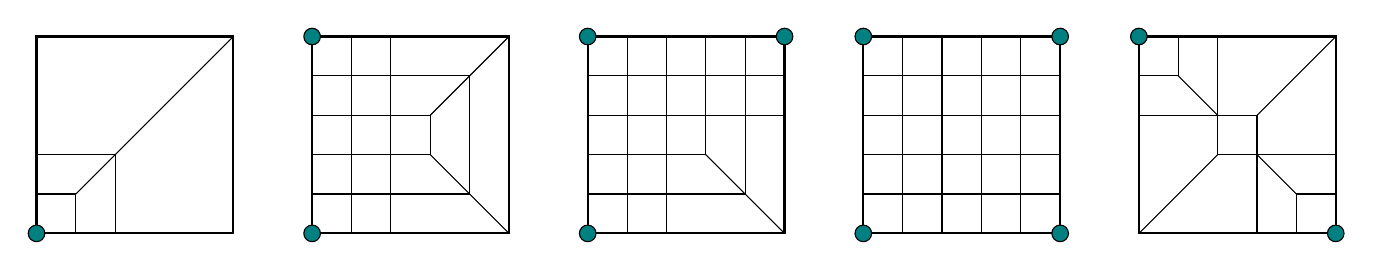
\begin{tikzpicture}
%\draw[step=0.5cm,gray,very thin] (0,0) grid (17,5); %background grid


\draw[thick] (0.5,0.5) rectangle (3,3);
\draw[](0.5,1)--(1,1)--(1,0.5);
\draw[](0.5,1.5)--(1.5,1.5)--(1.5,0.5);
\draw[](1,1)--(3,3);
\draw[black,fill=teal] (0.5,0.5) circle (3pt);


\draw[thick] (4,0.5) rectangle (6.5,3);
\draw[](4.5,0.5)--(4.5,3);
\draw[](5,0.5)--(5,3);
\draw[](4,1.5)--(5.5,1.5)--(5.5,2)--(4,2);
\draw[](4,1)--(6,1)--(6,2.5)--(4,2.5);
\draw[](5.5,2)--(6.5,3);
\draw[](5.5,1.5)--(6.5,0.5);
\draw[black,fill=teal] (4,0.5) circle (3pt);
\draw[black,fill=teal] (4,3) circle (3pt);

\draw[thick] (7.5,0.5) rectangle (10,3);
\draw[](8,0.5)--(8,3);
\draw[](8.5,0.5)--(8.5,3);
\draw[](7.5,2.5)--(10,2.5);
\draw[](7.5,2)--(10,2);
\draw[](7.5,1.5)--(9,1.5)--(9,3);
\draw[](7.5,1)--(9.5,1)--(9.5,3);
\draw[](9,1.5)--(10,0.5);
\draw[black,fill=teal] (7.5,0.5) circle (3pt);
\draw[black,fill=teal] (7.5,3) circle (3pt);
\draw[black,fill=teal] (10,3) circle (3pt);

\draw[thick] (11,0.5) rectangle (13.5,3);
\draw[](11,1)--(13.5,1);
\draw[](11,1.5)--(13.5,1.5);
\draw[](11,2)--(13.5,2);
\draw[](11,2.5)--(13.5,2.5);
\draw[](11.5,0.5)--(11.5,3);
\draw[](12,0.5)--(12,3);
\draw[](12.5,0.5)--(12.5,3);
\draw[](13,0.5)--(13,3);
\draw[black,fill=teal] (11,0.5) circle (3pt);
\draw[black,fill=teal] (11,3) circle (3pt);
\draw[black,fill=teal] (13.5,3) circle (3pt);
\draw[black,fill=teal] (13.5,0.5) circle (3pt);

\draw[thick] (14.5,0.5) rectangle (17,3);
\draw[black,fill=teal] (14.5,3) circle (3pt);
\draw[black,fill=teal] (17,0.5) circle (3pt);
\draw[](14.5,0.5)--(15.5,1.5);
\draw[](16,2)--(17,3);
\draw[](15.5,1.5) rectangle (16,2);
\draw[](14.5,2.5)--(15,2.5)--(15,3);
\draw[](14.5,2)--(15.5,2)--(15.5,3);
\draw[](15,2.5)--(15.5,2);
\draw[](16,1.5)--(16.5,1);
\draw[](16.5,0.5)--(16.5,1)--(17,1);
\draw[](16,0.5)--(16,1.5)--(17,1.5);

\end{tikzpicture}



\end{center}

After running the code, various vtu files are to be found in the OUT folder.

%................................................................
\paragraph{Case test=0}

\begin{center}

\includegraphics[width=6cm]{python_codes/fieldstone_102/results/test0/mesh1}
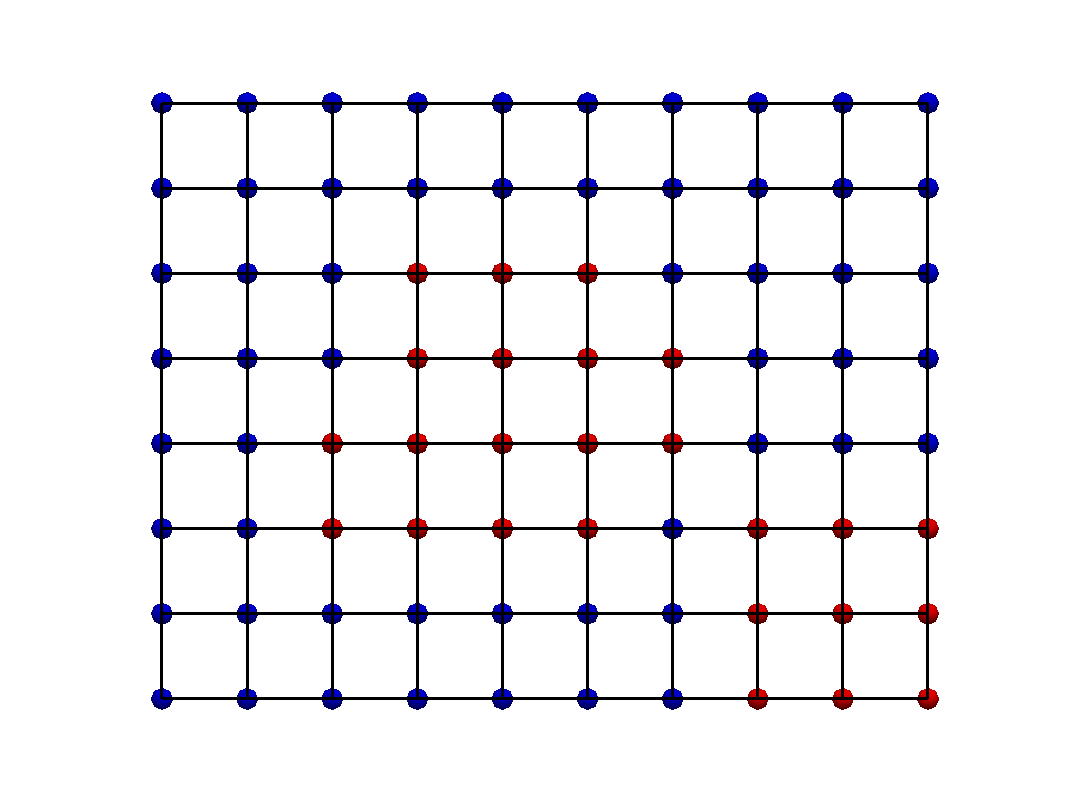
\includegraphics[width=6cm]{python_codes/fieldstone_102/results/test0/mesh2}\\
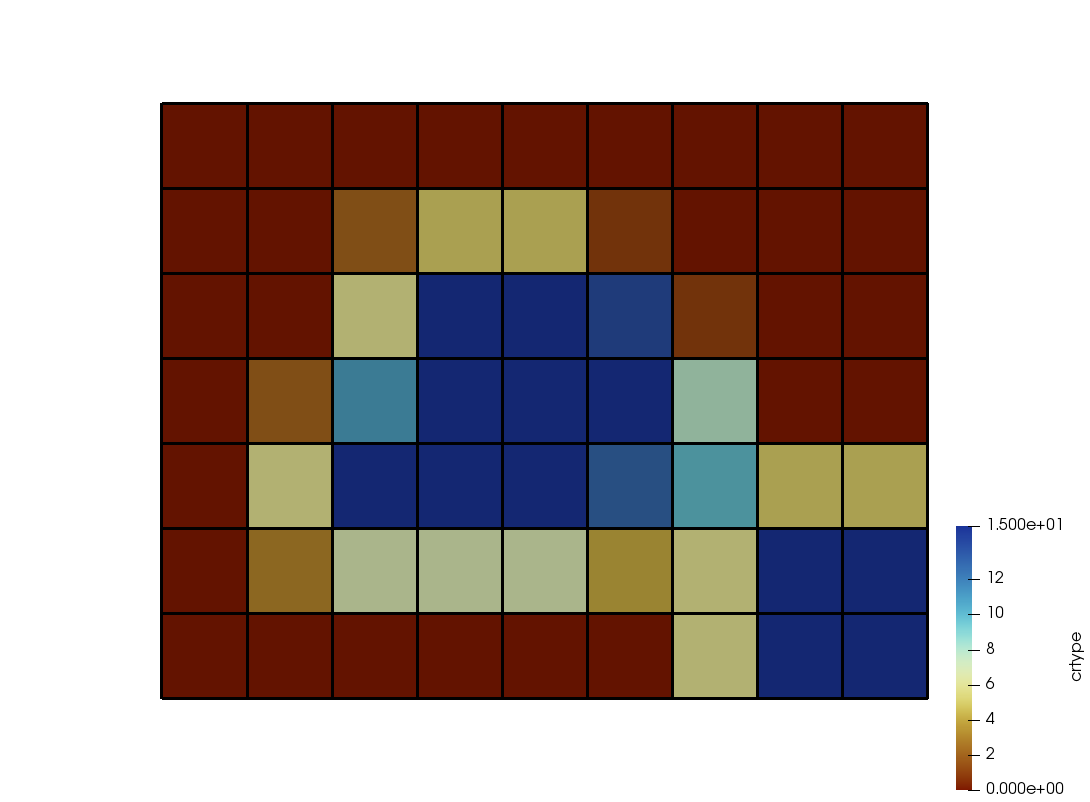
\includegraphics[width=6cm]{python_codes/fieldstone_102/results/test0/mesh3}
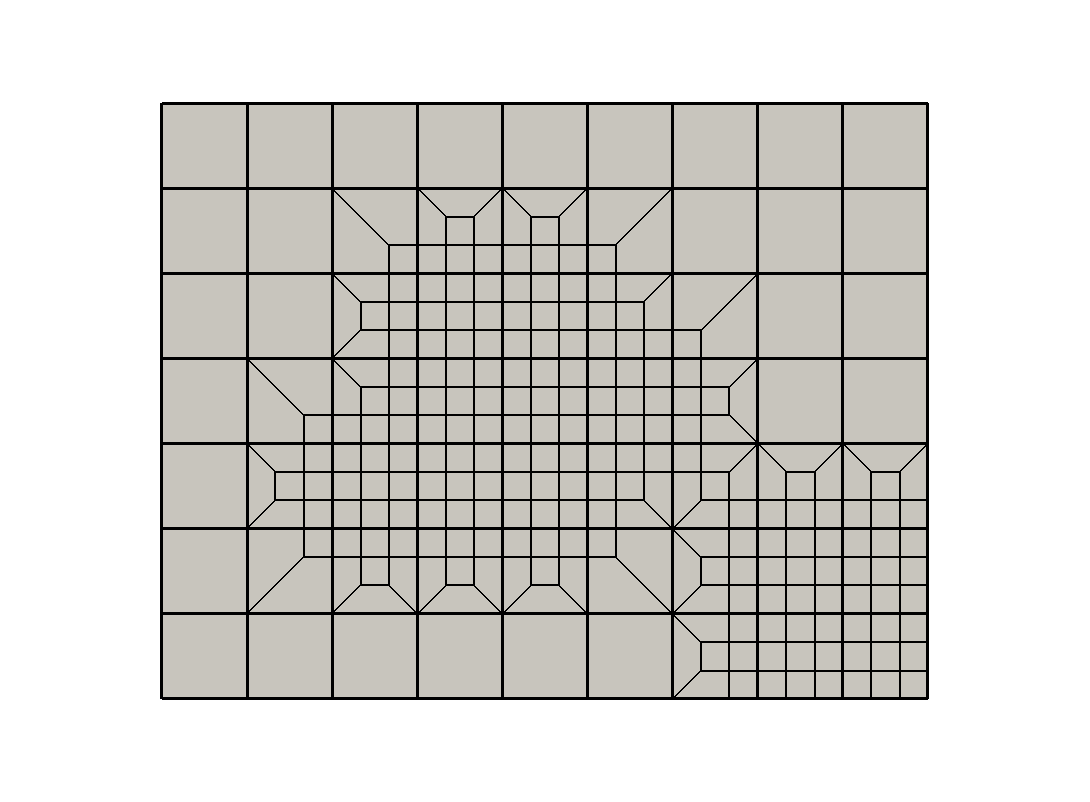
\includegraphics[width=6cm]{python_codes/fieldstone_102/results/test0/mesh4}\\
{\captionfont opla}
\end{center}

%................................................................
\paragraph{Case test=1}

\begin{center}
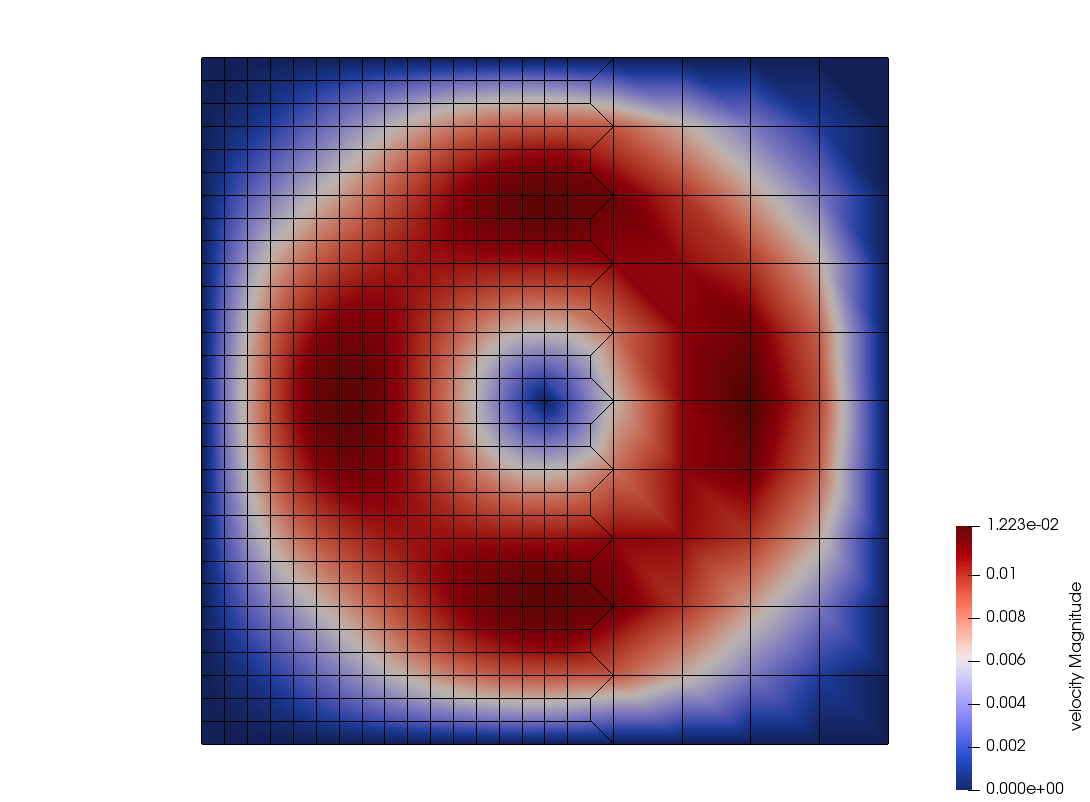
\includegraphics[width=6cm]{python_codes/fieldstone_102/results/test1/vel}
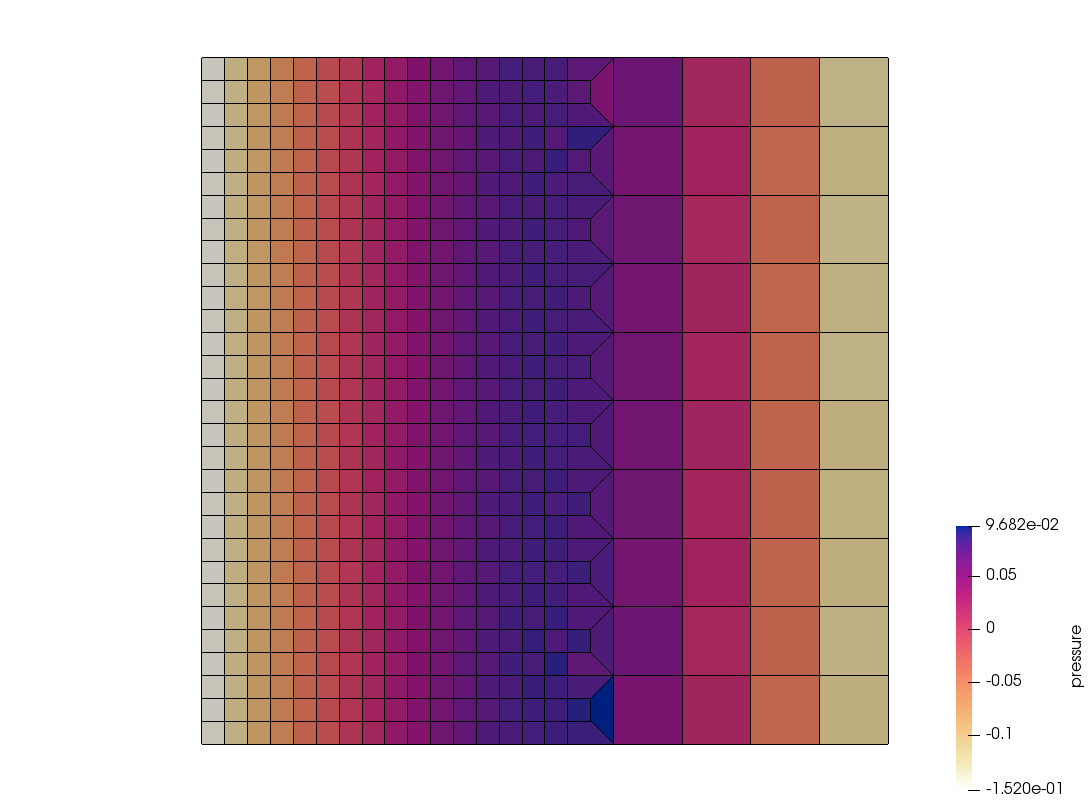
\includegraphics[width=6cm]{python_codes/fieldstone_102/results/test1/press}\\
{\captionfont Initial resolution 10x10}
\end{center}

%................................................................
\paragraph{Case test=2}

\begin{center}
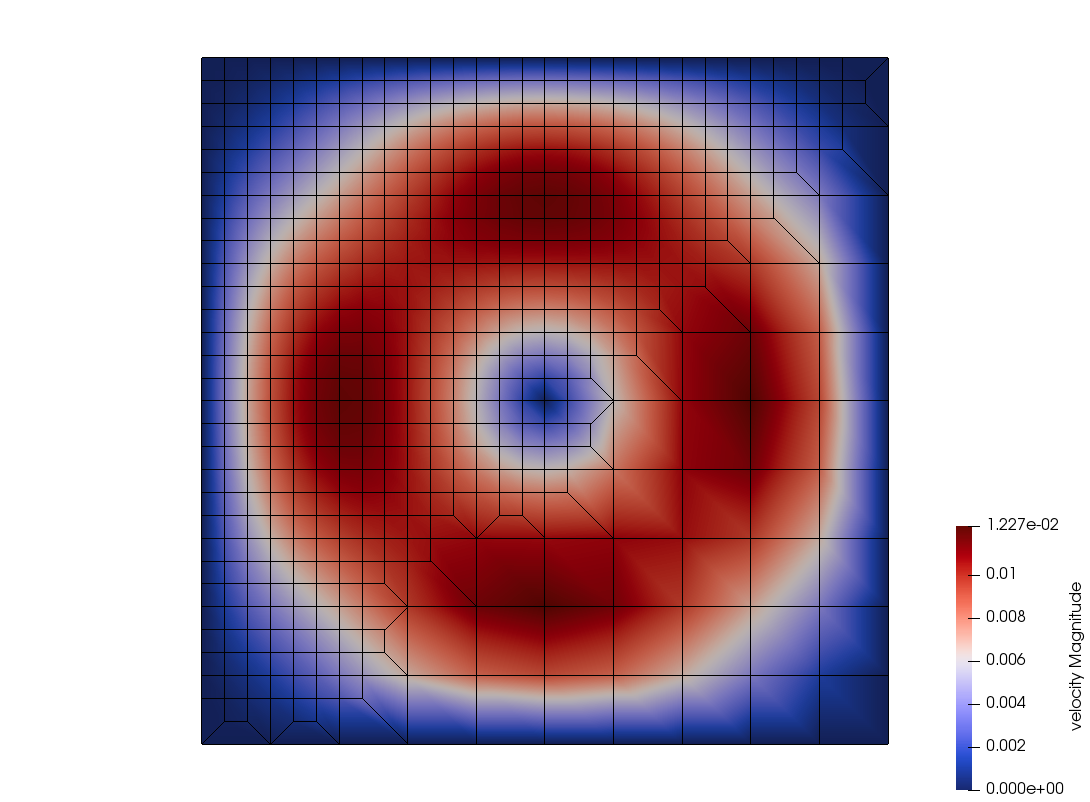
\includegraphics[width=6cm]{python_codes/fieldstone_102/results/test2/vel}
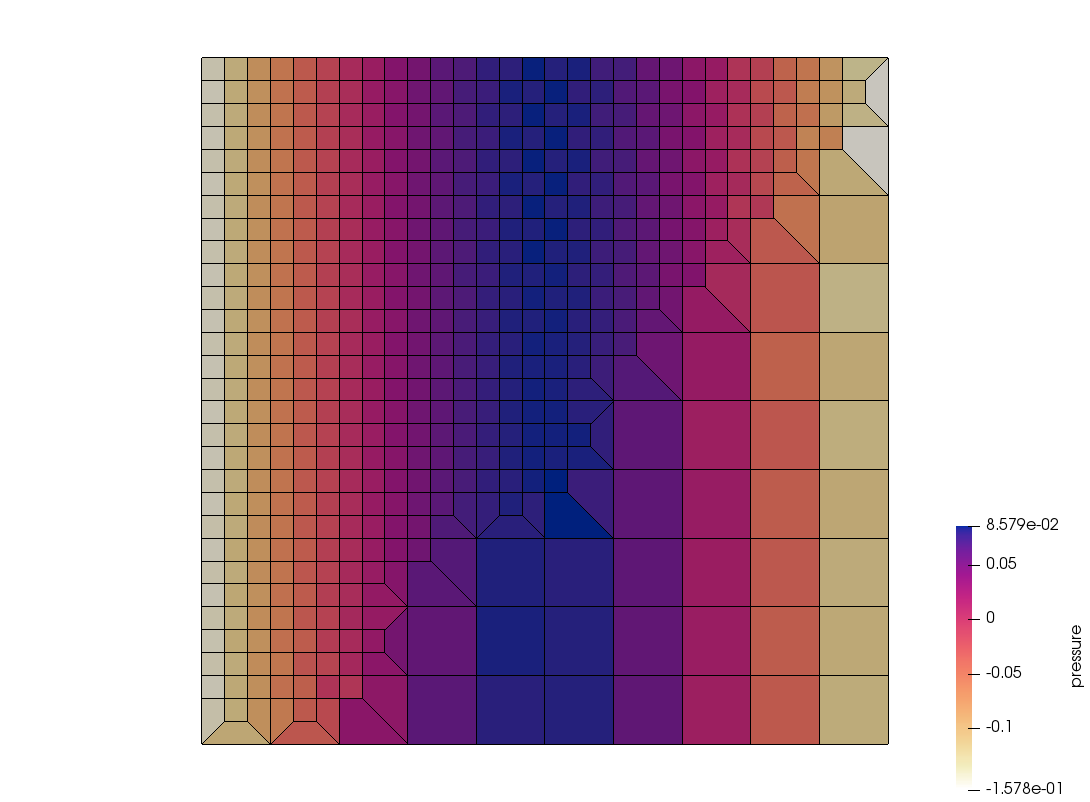
\includegraphics[width=6cm]{python_codes/fieldstone_102/results/test2/press}\\
{\captionfont Initial resolution 10x10}
\end{center}


%................................................................
\paragraph{Case test=3}

\begin{center}
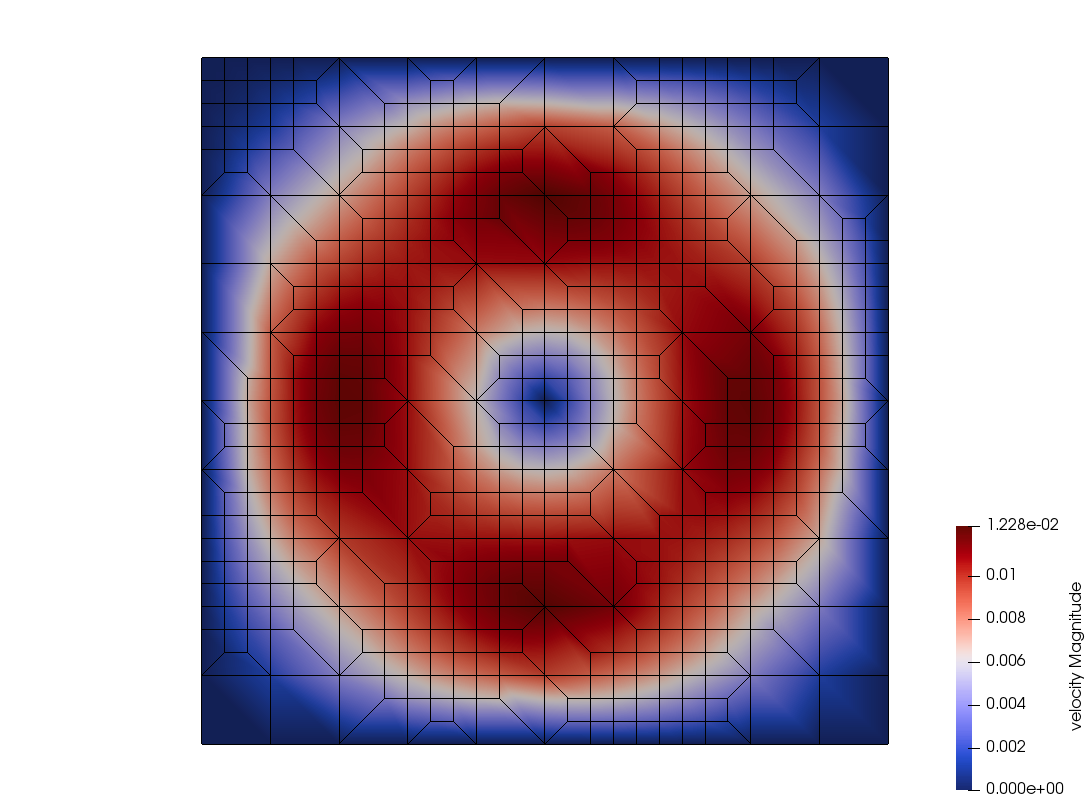
\includegraphics[width=6cm]{python_codes/fieldstone_102/results/test3/vel}
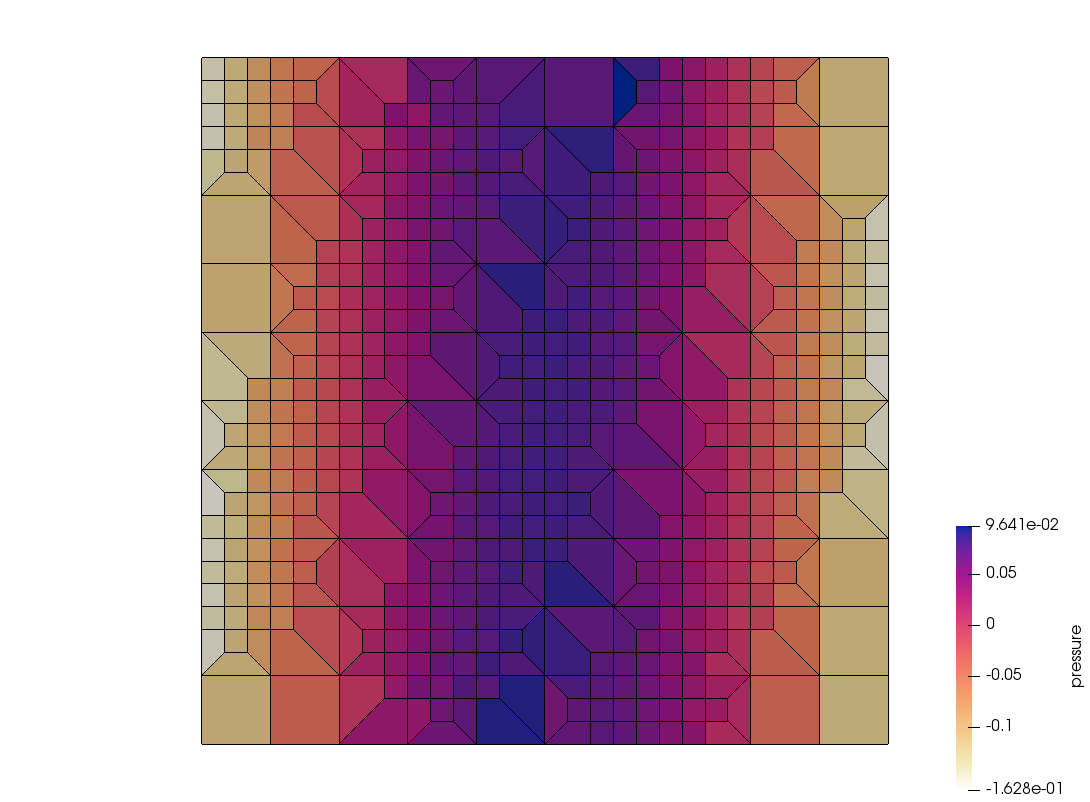
\includegraphics[width=6cm]{python_codes/fieldstone_102/results/test3/press}\\
{\captionfont Initial resolution 10x10}
\end{center}
















